Wu et al.'s method \cite{wu2025pihm} is tested here against its own record. Each panel of their Figs~3--7 is rebuilt with their choices as printed and with the standard form's, and each claim we tested, their circuits and filter included, is given a verdict with the computation or derivation behind it. Unless a tier is named, every number is an exact classical computation on the assembled residual: the ground state is the smallest right singular vector of the stacked residual (\Cref{sec:pipeline-reference}), errors are $L^\infty$ on 1001 points ($101\times101$ on two axes), and a dagger marks a ground state that is not trusted.

\subsection{The paper-faithful variant}
\label{app:faithful-conventions}

The paper-faithful variant is a panel with every choice Wu et al.\ print, and it runs only in this appendix. It shares with the standard form the conventions that fix Wu et al.'s matrices: the state holds the solution's coefficients in the normalised Chebyshev basis; every rank-one row uses the feature vector $\tau(x)$ unnormalised; $\G$ is the upper-triangular matrix acting on coefficients, the transpose of the $\mathbb{G}_n$ Wu et al.\ print; a polynomial coefficient or source enters through the lifts $\M_{x^p}$ from $n$ to $n+1$ qubits; an invariant constraint on a derivative is the row $\Brow(x_m)\G^{j}$; and $H$ is the Gram sum of \Cref{eq:pihm-hamiltonian}, which equals $R^\dagger R$ for the residual that stacks its operators. With these conventions the construction reproduces entry by entry the matrices $\G$, $\M_{x^p}$, $\nfold_1$ and $\Brow$ that Wu et al.'s supplementary material prints at $n=2$ (claim A-01), and the exact solution's $\eta_e=\|b\|^2$ (\Cref{eq:eta-e}) gives the printed scale factor of every ordinary panel (\Cref{tab:eta-reproduction}).

What the variant alone keeps is the data as printed. Its constraint points are rounded to two decimal places, $x_m=-0.2$, $x_z=-0.73$, $0.91$ and $x_m=-0.75$ on Figs~5a--5d and $x_z=0.02615$ on Fig.~7c, against the exact roots of \Cref{tab:catalogue-linear,tab:catalogue-nonlinear}. Its sources on Figs~5b--5d are Maclaurin polynomials of orders $\bar p=3$, $5$ and $7$. R3c and R3d keep the associated Legendre equation multiplied through by $1-x^2$, without the substitution of \Cref{app:legendre-substitution}. The partial differential panels keep the invariant sets of \Cref{tab:app-pde-invariants}, and the heat equation keeps its initial function at $t=0$. Where the printed choice is already exact (Fig.~3, Figs~4a and~4b, Fig.~7b) the variant is the problem as run, and Fig.~7's quadratic panels are carried by the doubled space in both (\Cref{sec:doubled-space}). Two choices that Wu et al.\ leave open are made alike in both variants. The datum point, not printed for Figs~3--6, is a point of the stated data where the solution does not vanish: $x_s=0$ on Figs~3b, 3d and~5, $x_s=1$ on Figs~4a and~4b, $x_s=\tfrac12$ on Figs~3c, 4c and~4d, and on two axes a point of the data slice where the stated function equals one, moved with the heat equation's data to $t=-1$ in the problem as run. The constraint $\mathcal T\bigl(\Brow(\pm1)\otimes I\bigr)$ is read as two rows, one for each sign.

\subsection{All panels}
\label{app:repro-panels}

\begin{table}[htbp]
    \centering
    \caption[Printed scale factors and errors of Wu et al.'s panels, as printed and as run]{\textbf{The exact solution reproduces the printed scale factor of every ordinary panel, to within one unit of the last printed digit, and of no partial differential or nonlinear panel.} Per panel of Wu et al.\ at their printed $n$: the printed scale factor $\eta$, the exact solution's $\eta_e=\|b\|^2$ ($b$, its Chebyshev coefficients; \Cref{eq:eta-e}) and the paper-faithful ground state's $\eta$; then the $L^\infty$ error of the panel as printed (the paper-faithful variant) and of the problem as run, at the printed $n$, and the problem's least error over $n$, on 1001 points ($101\times101$ on two axes). $^\dagger$Ground state not trusted (degenerate kernel, or gap ratio below 20); $^\ast$one unit low in the last printed digit; --, the doubled space (R6), whose kernel is never trusted. Classical computation.}
    \label{tab:eta-reproduction}
    \footnotesize
    \setlength{\tabcolsep}{3pt}
    \begin{tabular}{@{}l l r l l l c l l l@{}}
        \toprule
        & & & \multicolumn{4}{c}{Scale factor $\eta$} & \multicolumn{3}{c}{$L^\infty$ error} \\
        \cmidrule(lr){4-7}\cmidrule(l){8-10}
        Fig. & Problem & $n$ & Printed & Ideal $\eta_e$ & Ground state & Agrees & As printed & As run & As run, best ($n$) \\
        \midrule
        3b & R2a & 3 & 1.29 & \res[places=5]{build/R2a/faithful/standard/n3}{eta_ideal} & $\res[places=5]{build/R2a/faithful/standard/n3}{eta}\resflag{build/R2a/faithful/standard/n3}{trusted}{}{^{\dagger}}$ & \checkmark & $\res[2,sci]{build/R2a/faithful/standard/n3}{field_err_linf}\resflag{build/R2a/faithful/standard/n3}{trusted}{}{^{\dagger}}$ & $\res[2,sci]{build/R2a/standard/n3}{field_err_linf}\resflag{build/R2a/standard/n3}{trusted}{}{^{\dagger}}$ & \res[2,sci]{build/R2a/standard/best}{field_err_linf} ($n = \res{build/R2a/standard/best}{n}$) \\
        3c & R2b & 3 & 32.47 & \res[places=5]{build/R2b/faithful/standard/n3}{eta_ideal} & $\res[places=5]{build/R2b/faithful/standard/n3}{eta}\resflag{build/R2b/faithful/standard/n3}{trusted}{}{^{\dagger}}$ & \checkmark$^\ast$ & $\res[2,sci]{build/R2b/faithful/standard/n3}{field_err_linf}\resflag{build/R2b/faithful/standard/n3}{trusted}{}{^{\dagger}}$ & $\res[2,sci]{build/R2b/standard/n3}{field_err_linf}\resflag{build/R2b/standard/n3}{trusted}{}{^{\dagger}}$ & \res[2,sci]{build/R2b/standard/best}{field_err_linf} ($n = \res{build/R2b/standard/best}{n}$) \\
        3d & R2c & 5 & 451.71 & \res[places=5]{build/R2c/faithful/standard/n5}{eta_ideal} & $\res[places=5]{build/R2c/faithful/standard/n5}{eta}\resflag{build/R2c/faithful/standard/n5}{trusted}{}{^{\dagger}}$ & \checkmark & $\res[2,sci]{build/R2c/faithful/standard/n5}{field_err_linf}\resflag{build/R2c/faithful/standard/n5}{trusted}{}{^{\dagger}}$ & $\res[2,sci]{build/R2c/standard/n5}{field_err_linf}\resflag{build/R2c/standard/n5}{trusted}{}{^{\dagger}}$ & \res[2,sci]{build/R2c/standard/best}{field_err_linf} ($n = \res{build/R2c/standard/best}{n}$) \\
        4a & R3a & 3 & 1.75 & \res[places=5]{build/R3a/faithful/standard/n3}{eta_ideal} & $\res[places=5]{build/R3a/faithful/standard/n3}{eta}\resflag{build/R3a/faithful/standard/n3}{trusted}{}{^{\dagger}}$ & \checkmark & $\res[2,sci]{build/R3a/faithful/standard/n3}{field_err_linf}\resflag{build/R3a/faithful/standard/n3}{trusted}{}{^{\dagger}}$ & $\res[2,sci]{build/R3a/standard/n3}{field_err_linf}\resflag{build/R3a/standard/n3}{trusted}{}{^{\dagger}}$ & \res[2,sci]{build/R3a/standard/best}{field_err_linf} ($n = \res{build/R3a/standard/best}{n}$) \\
        4b & R3b & 3 & 1.49 & \res[places=5]{build/R3b/faithful/standard/n3}{eta_ideal} & $\res[places=5]{build/R3b/faithful/standard/n3}{eta}\resflag{build/R3b/faithful/standard/n3}{trusted}{}{^{\dagger}}$ & \checkmark & $\res[2,sci]{build/R3b/faithful/standard/n3}{field_err_linf}\resflag{build/R3b/faithful/standard/n3}{trusted}{}{^{\dagger}}$ & $\res[2,sci]{build/R3b/standard/n3}{field_err_linf}\resflag{build/R3b/standard/n3}{trusted}{}{^{\dagger}}$ & \res[2,sci]{build/R3b/standard/best}{field_err_linf} ($n = \res{build/R3b/standard/best}{n}$) \\
        4c & R3c & 5 & 108.51 & \res[places=5]{build/R3c/faithful/standard/n5}{eta_ideal} & $\res[places=5]{build/R3c/faithful/standard/n5}{eta}\resflag{build/R3c/faithful/standard/n5}{trusted}{}{^{\dagger}}$ & \checkmark & $\res[2,sci]{build/R3c/faithful/standard/n5}{field_err_linf}\resflag{build/R3c/faithful/standard/n5}{trusted}{}{^{\dagger}}$ & $\res[2,sci]{build/R3c/standard/n5}{field_err_linf}\resflag{build/R3c/standard/n5}{trusted}{}{^{\dagger}}$ & \res[2,sci]{build/R3c/standard/best}{field_err_linf} ($n = \res{build/R3c/standard/best}{n}$) \\
        4d & R3d & 5 & 135.38 & \res[places=5]{build/R3d/faithful/standard/n5}{eta_ideal} & $\res[places=5]{build/R3d/faithful/standard/n5}{eta}\resflag{build/R3d/faithful/standard/n5}{trusted}{}{^{\dagger}}$ & \checkmark & $\res[2,sci]{build/R3d/faithful/standard/n5}{field_err_linf}\resflag{build/R3d/faithful/standard/n5}{trusted}{}{^{\dagger}}$ & $\res[2,sci]{build/R3d/standard/n5}{field_err_linf}\resflag{build/R3d/standard/n5}{trusted}{}{^{\dagger}}$ & \res[2,sci]{build/R3d/standard/best}{field_err_linf} ($n = \res{build/R3d/standard/best}{n}$) \\
        5a & R4a & 3 & 1.35 & \res[places=5]{build/R4a/faithful/standard/n3}{eta_ideal} & $\res[places=5]{build/R4a/faithful/standard/n3}{eta}\resflag{build/R4a/faithful/standard/n3}{trusted}{}{^{\dagger}}$ & \checkmark & $\res[2,sci]{build/R4a/faithful/standard/n3}{field_err_linf}\resflag{build/R4a/faithful/standard/n3}{trusted}{}{^{\dagger}}$ & $\res[2,sci]{build/R4a/standard/n3}{field_err_linf}\resflag{build/R4a/standard/n3}{trusted}{}{^{\dagger}}$ & \res[2,sci]{build/R4a/standard/best}{field_err_linf} ($n = \res{build/R4a/standard/best}{n}$) \\
        5b & R4b & 3 & 14.74 & \res[places=5]{build/R4b/faithful/standard/n3}{eta_ideal} & $\res[places=5]{build/R4b/faithful/standard/n3}{eta}\resflag{build/R4b/faithful/standard/n3}{trusted}{}{^{\dagger}}$ & \checkmark$^\ast$ & $\res[2,sci]{build/R4b/faithful/standard/n3}{field_err_linf}\resflag{build/R4b/faithful/standard/n3}{trusted}{}{^{\dagger}}$ & $\res[2,sci]{build/R4b/standard/n3}{field_err_linf}\resflag{build/R4b/standard/n3}{trusted}{}{^{\dagger}}$ & \res[2,sci]{build/R4b/standard/best}{field_err_linf} ($n = \res{build/R4b/standard/best}{n}$) \\
        5c & R4c & 4 & 0.82 & \res[places=5]{build/R4c/faithful/standard/n4}{eta_ideal} & $\res[places=5]{build/R4c/faithful/standard/n4}{eta}\resflag{build/R4c/faithful/standard/n4}{trusted}{}{^{\dagger}}$ & \checkmark & $\res[2,sci]{build/R4c/faithful/standard/n4}{field_err_linf}\resflag{build/R4c/faithful/standard/n4}{trusted}{}{^{\dagger}}$ & $\res[2,sci]{build/R4c/standard/n4}{field_err_linf}\resflag{build/R4c/standard/n4}{trusted}{}{^{\dagger}}$ & \res[2,sci]{build/R4c/standard/best}{field_err_linf} ($n = \res{build/R4c/standard/best}{n}$) \\
        5d & R4d & 4 & 77.51 & \res[places=5]{build/R4d/faithful/standard/n4}{eta_ideal} & $\res[places=5]{build/R4d/faithful/standard/n4}{eta}\resflag{build/R4d/faithful/standard/n4}{trusted}{}{^{\dagger}}$ & \checkmark & $\res[2,sci]{build/R4d/faithful/standard/n4}{field_err_linf}\resflag{build/R4d/faithful/standard/n4}{trusted}{}{^{\dagger}}$ & $\res[2,sci]{build/R4d/standard/n4}{field_err_linf}\resflag{build/R4d/standard/n4}{trusted}{}{^{\dagger}}$ & \res[2,sci]{build/R4d/standard/best}{field_err_linf} ($n = \res{build/R4d/standard/best}{n}$) \\
        \midrule
        6b & R5a & 3 & 5.21559 & \res[places=5]{build/R5a/faithful/standard/n3x3}{eta_ideal} & $\res[places=5]{build/R5a/faithful/standard/n3x3}{eta}\resflag{build/R5a/faithful/standard/n3x3}{trusted}{}{^{\dagger}}$ & $\times$ & $\res[2,sci]{build/R5a/faithful/standard/n3x3}{field_err_linf}\resflag{build/R5a/faithful/standard/n3x3}{trusted}{}{^{\dagger}}$ & $\res[2,sci]{build/R5a/standard/n3x3}{field_err_linf}\resflag{build/R5a/standard/n3x3}{trusted}{}{^{\dagger}}$ & \res[2,sci]{build/R5a/standard/best}{field_err_linf} ($n = \res{build/R5a/standard/best}{n}$) \\
        6d & R5b & 4 & 603.863 & \res[places=5]{build/R5b/faithful/standard/n4x4}{eta_ideal} & $\res[places=5]{build/R5b/faithful/standard/n4x4}{eta}\resflag{build/R5b/faithful/standard/n4x4}{trusted}{}{^{\dagger}}$ & $\times$ & $\res[2,sci]{build/R5b/faithful/standard/n4x4}{field_err_linf}\resflag{build/R5b/faithful/standard/n4x4}{trusted}{}{^{\dagger}}$ & $\res[2,sci]{build/R5b/standard/n4x4}{field_err_linf}\resflag{build/R5b/standard/n4x4}{trusted}{}{^{\dagger}}$ & \res[2,sci]{build/R5b/standard/best}{field_err_linf} ($n = \res{build/R5b/standard/best}{n}$) \\
        6f & R5c & 5 & 216.469 & \res[places=5]{build/R5c/faithful/standard/n5x5}{eta_ideal} & $\res[places=5]{build/R5c/faithful/standard/n5x5}{eta}\resflag{build/R5c/faithful/standard/n5x5}{trusted}{}{^{\dagger}}$ & $\times$ & $\res[2,sci]{build/R5c/faithful/standard/n5x5}{field_err_linf}\resflag{build/R5c/faithful/standard/n5x5}{trusted}{}{^{\dagger}}$ & $\res[2,sci]{build/R5c/standard/n5x5}{field_err_linf}\resflag{build/R5c/standard/n5x5}{trusted}{}{^{\dagger}}$ & \res[2,sci]{build/R5c/standard/best}{field_err_linf} ($n = \res{build/R5c/standard/best}{n}$) \\
        7b & R6a & 2 & 3.75367 & \res[places=5]{build/R6a/faithful/standard/n2}{eta_ideal} & $\res[places=5]{build/R6a/faithful/standard/n2}{eta}\resflag{build/R6a/faithful/standard/n2}{trusted}{}{^{\dagger}}$ & $\times$ & $\res[2,sci]{build/R6a/faithful/standard/n2}{field_err_linf}\resflag{build/R6a/faithful/standard/n2}{trusted}{}{^{\dagger}}$ & $\res[2,sci]{build/R6a/standard/n2}{field_err_linf}\resflag{build/R6a/standard/n2}{trusted}{}{^{\dagger}}$ & -- \\
        7c & R6b & 2 & 0.07984 & \res[places=5]{build/R6b/faithful/standard/n2}{eta_ideal} & $\res[places=5]{build/R6b/faithful/standard/n2}{eta}\resflag{build/R6b/faithful/standard/n2}{trusted}{}{^{\dagger}}$ & $\times$ & $\res[2,sci]{build/R6b/faithful/standard/n2}{field_err_linf}\resflag{build/R6b/faithful/standard/n2}{trusted}{}{^{\dagger}}$ & $\res[2,sci]{build/R6b/standard/n2}{field_err_linf}\resflag{build/R6b/standard/n2}{trusted}{}{^{\dagger}}$ & -- \\
        \bottomrule
    \end{tabular}
\end{table}

Only the ordinary panels' scale factors reproduce, and the agreement is the exact solution's; as printed, the panels' own ground states fall short of it. R2b, R3c and R3d have no trusted ground state at the printed $n$. R3c and R3d, multiplied through by $1-x^2$, have solutions with a branch point at each end, which a Chebyshev series approximates only algebraically (\Cref{app:legendre-substitution}), and Fig.~5's panels hold at the floors of \Cref{app:repro-triage}. As run, every ordinary problem converges spectrally until the standard form's conditioning stops it. Wedin's bound $\epsilon_{\mathrm{mach}}\sigma_{\max}/(\sigma_1-\sigma_0)$ (\Cref{prop:wedin}) grows by a factor of about $16$ per qubit on a second-order equation with constant coefficients, whose $\sigma_{\max}$ grows as $N^4$, so the least error is reached between $n=3$ and $6$ and the error rises beyond it, to \res[2,sci]{build/R2a/standard/n10}{field_err_linf} on R2a at $n=10$. The partial differential and doubled-space panels reproduce no printed scale factor, by the exact solution or by any ground state (\Cref{app:repro-unreproduced}).

\subsection{The Fig.~5 triage}
\label{app:repro-triage}

\begin{figure}[htbp]
    \centering
    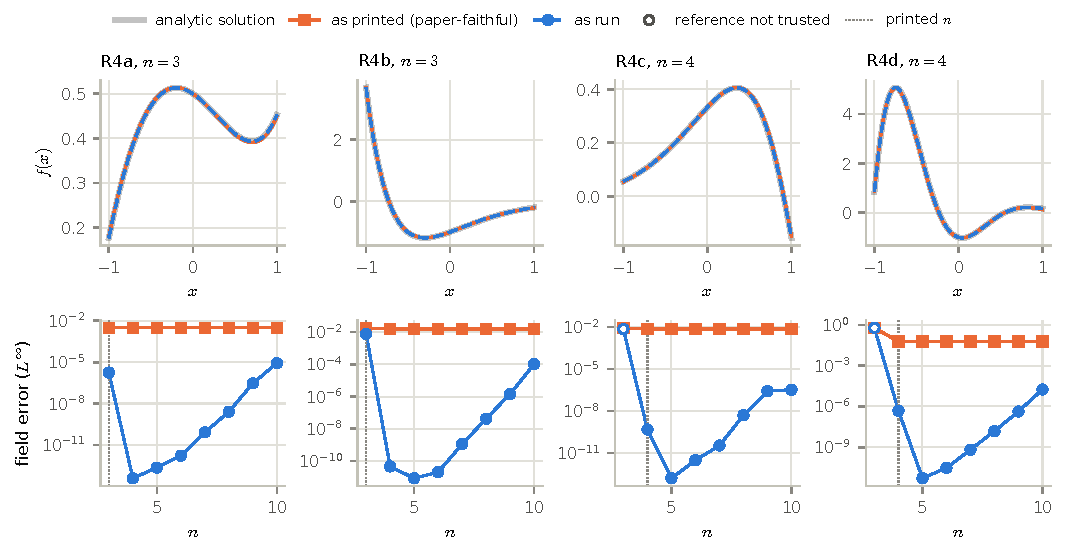
\includegraphics[width=\linewidth]{Figs/faithful_vs_corrected.pdf}
    \caption[The paper-faithful variant against the problems as run, Fig.~5]{\textbf{As printed, each panel of Wu et al.'s Fig.~5 holds at an error floor that no resolution removes; as run, it converges spectrally.} R4a--R4d. Top: the analytic solution, the paper-faithful ground state (rounded constraint point, Maclaurin source) and the problem as run (exact root, Chebyshev source) at the printed $n$; the three coincide at plot scale, the paper-faithful errors there lying between $\res[2,sci]{build/R4a/faithful/standard/n3}{field_err_linf}$ (R4a) and $\res[2,sci]{build/R4d/faithful/standard/n4}{field_err_linf}$ (R4d). Bottom: the $L^\infty$ field error against $n$ for both variants (open where the reference is not trusted), the printed $n$ dotted. The paper-faithful error holds at its floor (\Cref{tab:app-fig5-triage}); as run it falls to between $\res[2,sci]{build/R4a/standard/best}{field_err_linf}$ and $\res[2,sci]{build/R4b/standard/best}{field_err_linf}$ at $n=4$ or $5$, then rises with the standard form's conditioning (\Cref{prop:wedin}). On R4b the printed $n=3$ is itself under-resolved: as run, the error there is $\res[2,sci]{build/R4b/standard/n3}{field_err_linf}$. Classical computation (dense \gls{svd}).}
    \label{fig:faithful-vs-corrected}
\end{figure}

\begin{table}[htbp]
    \centering
    \caption[The printed choices behind the error of Wu et al.'s Fig.~5]{\textbf{Each printed choice alone sets an error floor; only both departures together converge.} $L^\infty$ error on Wu et al.'s Fig.~5 panels over $n=4,\dots,10$: the paper-faithful variant (rounded constraint point, Maclaurin source), each departure alone (exact root; Chebyshev source coefficients), and both together at their best $n$. --, R4a's polynomial source is already exact, so its rounded point acts alone. Classical computation.}
    \label{tab:app-fig5-triage}
    \small
    \begin{tabular}{@{}l l l l l l@{}}
        \toprule
        Fig. & Problem & Faithful & Exact root & Chebyshev source & Both, best \\
        \midrule
        5a & R4a & \res[2,sci]{build/R4a/faithful/standard/floor}{low} & -- & -- & \res[2,sci]{build/R4a/standard/best}{field_err_linf} ($n = \res{build/R4a/standard/best}{n}$) \\
        5b & R4b & \res[2,sci]{build/R4b/faithful/standard/floor}{low} & \res[2,sci]{build/R4b/faithful/standard/floor/exact-root}{low} & \res[2,sci]{build/R4b/faithful/standard/floor/chebyshev-source}{low} & \res[2,sci]{build/R4b/standard/best}{field_err_linf} ($n = \res{build/R4b/standard/best}{n}$) \\
        5c & R4c & \res[2,sci]{build/R4c/faithful/standard/floor}{low} & \res[2,sci]{build/R4c/faithful/standard/floor/exact-root}{low} & \res[2,sci]{build/R4c/faithful/standard/floor/chebyshev-source}{low} & \res[2,sci]{build/R4c/standard/best}{field_err_linf} ($n = \res{build/R4c/standard/best}{n}$) \\
        5d & R4d & \res[2,sci]{build/R4d/faithful/standard/floor}{low} & \res[2,sci]{build/R4d/faithful/standard/floor/exact-root}{low} & \res[2,sci]{build/R4d/faithful/standard/floor/chebyshev-source}{low} & \res[2,sci]{build/R4d/standard/best}{field_err_linf} ($n = \res{build/R4d/standard/best}{n}$) \\
        \bottomrule
    \end{tabular}
\end{table}

R4a's source is a polynomial, represented exactly, so its rounded point acts alone: the printed $f'(-0.2)=0$ stands for an extremum at $x\approx-0.196$, and the error holds at \res[2,sci]{build/R4a/faithful/standard/floor}{high} for every $n$ from 4 to 10, against \res[2,sci]{build/R4a/standard/best}{field_err_linf} at $n=\res{build/R4a/standard/best}{n}$ at the exact point. On R4b to R4d each printed choice alone sets a floor, and only both departures together converge. The source dominates on R4d, whose order-7 Maclaurin polynomial departs from the source near $x=-1$ by more than the source's own largest value: with the exact root, raising the order to 11 and to 15 lowers the error at $n=4$ from \res[2,sci]{build/R4d/standard/n4/maclaurin-7}{field_err_linf} to \res[2,sci]{build/R4d/standard/n4/maclaurin-11}{field_err_linf} and \res[2,sci]{build/R4d/standard/n4/maclaurin-15}{field_err_linf}, against \res[2,sci]{build/R4d/standard/n4}{field_err_linf} with the Chebyshev source.

\subsection{Panels not reproduced, and printed errors}
\label{app:repro-unreproduced}

\paragraph{Printed errors.} Wu et al.\ print the solution of their Laplace example as $\operatorname{csch}\pi\,\cosh(\pi x/2)\sinh(\pi(y+1)/2)$ (claim A-05). It is not harmonic, its two second derivatives summing to $\tfrac{\pi^2}{2}f$, and it violates $f(\pm1,y)=0$, since $\cosh(\pi/2)\ne0$. The solution, and the reference throughout, is $\cos(\pi x/2)\sinh(\pi(y+1)/2)/\sinh\pi$. The printed scale factor was not computed from the printed form either, which gives $\eta_e=\prov{48.57}$ at $n=(3,3)$. Wu et al.'s heat data, stated at $t=0$ inside the time domain $[-1,1]$, pose a backward heat problem on $[-1,0]$ (\Cref{app:datum-slice}).

\begin{table}[htbp]
    \centering
    \caption[Wu et al.'s invariant sets for their partial differential examples]{\textbf{Each of Wu et al.'s invariant sets for their partial differential examples admits a family of solutions, which the truncation suppresses only near the printed resolution.} The constraints Wu et al.\ impose on Laplace's equation (R5a, their Fig.~6b), the heat equation $f_t=\tfrac1{25}f_{xx}$ (R5b, Fig.~6d) and the wave equation $f_{tt}=4f_{xx}$ (R5c, Fig.~6f); the solutions that satisfy the equation and every constraint, $\ell$ a positive integer and $\phi_\ell$ a phase fixed by the constraints in $t$; the printed $n$ per axis; and the least $n$ per axis above the printed one at which the paper-faithful residual's near-kernel is degenerate, with its dimension. Classical computation (dense \gls{svd}).}
    \label{tab:app-pde-invariants}
    \small
    \begin{tabular}{@{}l l l c l@{}}
        \toprule
        Problem & Printed invariant set & Solutions satisfying it & Printed $n$ & Degenerate from \\
        \midrule
        R5a & $f(\pm1,y)=0$, $f(x,-1)=0$ & $\sin\tfrac{\ell\pi(x+1)}{2}\,\sinh\tfrac{\ell\pi(y+1)}{2}$ & $3$ & $(5,5)$, dimension \res{build/R5a/faithful/standard/n5x5}{kernel_dimension} \\
        R5b & $f(t,\pm1)=0$, $\partial_xf(t,\pm\tfrac34)=0$ & $\sin\tfrac{\ell\pi(x+1)}{2}\,e^{-(\ell\pi/2)^2t/25}$, $\ell\equiv4\pmod 8$ & $4$ & $(6,6)$, dimension \res{build/R5b/faithful/standard/n6x6}{kernel_dimension} \\
        R5c & $f(\tfrac18,x)=f(\tfrac78,x)=0$, $f(t,\pm1)=0$ & $\sin\tfrac{\ell\pi(x+1)}{2}\,\cos(\ell\pi t+\phi_\ell)$, $4\mid\ell$ & $5$ & $(6,6)$, dimension \res{build/R5c/faithful/standard/n6x6}{kernel_dimension} \\
        \bottomrule
    \end{tabular}
\end{table}

\paragraph{The invariant sets.} None of Wu et al.'s sets for their partial differential examples contains the function that fixes the solution. Laplace's set omits the top side, and the heat and wave sets omit the initial function and place interior constraints at zeros of the known solution instead, $\partial_xf=0$ at $x=\pm\tfrac34$ and $f=0$ at $t=\tfrac18$ and $\tfrac78$, which a new problem would not supply. Each set therefore admits the family of \Cref{tab:app-pde-invariants}. At the printed resolution the truncation suppresses all but the solution's member, and the near-kernel is one-dimensional and trusted on all three panels. As $n$ grows the other members become representable and the near-kernel grows. On Laplace's equation the bottom of the spectrum is already near-degenerate at $n=(4,4)$, where the gap of $H$ relative to its norm is \res[2,sci]{build/R5a/faithful/standard/n4x4}{relative_gap}, and at $(5,5)$ the field error is \res[2]{build/R5a/faithful/standard/n5x5}{field_err_linf}; the heat and wave sets fail at $(6,6)$, with errors \res[2]{build/R5b/faithful/standard/n6x6}{field_err_linf} and \res[2]{build/R5c/faithful/standard/n6x6}{field_err_linf}. The datum slices of \Cref{app:datum-slice}, which impose the omitted function, leave on Laplace's equation a one-dimensional kernel trusted at every resolution computed from $n=(3,3)$ to $(6,6)$, with gap ratio \res[2,sci]{build/R5a/standard/n6x6}{gap_ratio} at the last, and on the heat equation, posed forward from $t=-1$, an error of \res[2,sci]{build/R5b/standard/n6x6}{field_err_linf} at $(6,6)$.

\paragraph{Fig.~6's scale factors.} The printed values are $5.21559$, $603.863$ and $216.469$; the exact solutions give \res[places=5]{build/R5a/faithful/standard/n3x3}{eta_ideal}, \res[places=5]{build/R5b/faithful/standard/n4x4}{eta_ideal} and \res[places=5]{build/R5c/faithful/standard/n5x5}{eta_ideal}, and the ground states at the printed $n$, trusted on all three, do not give the printed values either (\Cref{tab:eta-reproduction}). An unprinted datum point would explain Laplace's value alone: over a $41\times41$ grid of datum points its ground state's $\eta$ spans \prov{5.127} to \prov{5.261}, which contains the print, while the heat and wave ground states stay within \prov{598.58--599.14} and \prov{239.826--239.828}. Reading $\mathcal T\bigl(\Brow(\pm1)\otimes I\bigr)$ as one summed row degenerates the Laplace kernel and moves the heat and wave values further from the print, to \prov{727.47} and \prov{634.66}. A time domain of $[0,1]$ or $[0,2]$ in place of $[-1,1]$ gives \prov{38.4} or \prov{25.5} for heat and \prov{249.6} or \prov{239.8} for wave, and a neighbouring resolution gives \res{build/R5b/faithful/standard/n3x3}{eta_ideal} or \res{build/R5b/faithful/standard/n5x5}{eta_ideal} for heat and \res{build/R5c/faithful/standard/n4x4}{eta_ideal} or \res{build/R5c/faithful/standard/n6x6}{eta_ideal} for wave. Wu et al.'s own preparation, imaginary time from $\ket0$ under $H/\|H\|_F$ stopped at a finite time, does not reach the printed values: on Laplace's equation its $\eta$ falls monotonically to the ground state's, which lies above the print, and $\ket0$, the constant function, is orthogonal to the heat and wave solutions, which are odd in $x$. The one explanation left untested is a shot-sampled interferometric readout, whose noise would scatter the value; that readout was simulated with shots only at $n=(2,2)$ on Laplace's equation (\Cref{sec:pipeline-readout}), below every printed resolution. Laplace's value is consistent with an unprinted datum point, and the heat and wave values are unexplained.

\paragraph{Fig.~7's scale factors.} The doubled space has no unique ground state: at the printed $n=2$ its kernel has dimension \res{build/R6a/faithful/standard/n2}{kernel_dimension} on R6a and \res{build/R6b/faithful/standard/n2}{kernel_dimension} on R6b (claim A-10). We read out instead the product state $\hat b\otimes\hat b$ of least residual, the state Wu et al.\ describe their construction as selecting. On R6a, whose solution $1-x^2/8$ is represented exactly, it gives the exact solution's $\eta_e=\res[places=5]{build/R6a/faithful/standard/n2}{eta}$, and on R6b \res[places=5]{build/R6b/faithful/standard/n2}{eta} against the exact \res[places=5]{build/R6b/faithful/standard/n2}{eta_ideal}; the printed values are $3.75367$ and $0.07984$. Another datum point does not explain them: R6a's product state gives the same $\eta$ at every datum point tried, and R6b's spans \prov{0.0416--0.0479}. Nor does another resolution, since $\eta$ doubles with each qubit, to \res[places=5]{build/R6a/faithful/standard/n3}{eta} and \res[places=5]{build/R6a/faithful/standard/n4}{eta} on R6a and \res[places=5]{build/R6b/faithful/standard/n3}{eta} and \res[places=5]{build/R6b/faithful/standard/n4}{eta} on R6b at $n=3$ and $4$. The converged filter's output from $\ket0$, the projection of $\ket0$ onto the kernel, gives \prov{3.72756} on R6a and \prov{0.157} on R6b. Imaginary time from $\ket0$ under $H/\|H\|_F$, stopped at a finite time, passes through both printed values, at $\beta\approx\prov{178}$ and $\beta\approx\prov{302}$; Wu et al.\ print no time for Fig.~7, so this is consistent with their values without confirming them. The normalisation of the doubled-space readout (their Eq.~39) would need that readout, which was not built.

\subsection{Wu et al.'s claims}
\label{app:paper-claims}

\begin{table}[htbp]
    \centering
    \caption[The claims of Wu et al.\ tested, and their verdicts]{\textbf{The claims of Wu et al.\ \cite{wu2025pihm} that we tested, and their verdicts.} $\G$, differentiation matrix; $\M$, multiplication operator; $\nfold_1$, product-to-sum fold; $\Brow$, $\Dzero$, zero and collapse constraint rows; $\eta$, scale factor; $\beta$, imaginary time; $\lambda_{\max}$, $\lambda_2$, largest and second-smallest eigenvalues of $H$; $x_s$, datum point.}
    \label{tab:paper-claims}
    \small
    \begin{tabular}{@{}l p{0.52\linewidth} p{0.3\linewidth}@{}}
        \toprule
        & Claim & Verdict \\
        \midrule
        A-01 & $\G$, $\M$, $\nfold_1$ and $\Brow$ as printed at $n = 2$ & reproduced \\
        A-02 & the printed $\eta$ of Figs~3--5 (11 panels) & reproduced: within one unit of the last printed digit, nine of eleven equal when rounded \\
        A-03 & the printed $\eta$ of Fig.~6 & not reproduced \\
        A-04 & the printed $\eta$ of Fig.~7 & not reproduced \\
        A-05 & the printed Laplace solution & a typographical error ($\cosh$ for $\cos$) \\
        A-06 & the $\Brow$ circuit (Fig.~2): $n+2$ qubits, prefactor $\sqrt{2^{n+1}}$ & confirmed, exact \\
        A-07 & the $\G$ circuit (Fig.~9): $2n+3$ qubits, $O(n^3)$ gates, error decreasing exponentially & partly: the mechanism reproduced; built on $2n+5$ qubits; the error falls as about $N^{-5}$; the prefactor valid but loose (\Cref{app:published-resources}) \\
        A-08 & the $\Dzero$ circuit (Fig.~8): prefactor $\sqrt{2^{n+1}}/f(x_s)$ & confirmed, exact \\
        A-09 & the linear $H$ is positive definite with distinct eigenvalues & partly: positive semi-definite, an exact discrete solution being an exact kernel; the bottom need not be distinct \\
        A-10 & the doubled-space $H$ has at least $2^{2n-1}$ zero eigenvalues & confirmed: $\res{build/R6a/standard/n5}{kernel_count}$ on R6a at $n=5$, against $2^{2n-1}=512$ \\
        A-11 & the time rule $\beta \ge \lambda_{\max}/(\lambda_2(n-1))$ suffices & not met: short of the time for $\varepsilon$ by at least $(n-1)\ln(1/\varepsilon)$ (\Cref{eq:time-rule-shortfall}); misses $\varepsilon$ on every trusted record \\
        A-12 & the necessary terms scale as $O(\mathrm{poly}(n))$ and are efficient & partly: true of the gates, not of the subnormalisation \\
        A-13 & the examples are solved accurately at the printed $n$ & partly: Figs~4a and~4b to rounding; R2b, R3c and R3d not trusted; Fig.~5 held at the floors of its printed points and sources \\
        \bottomrule
    \end{tabular}
\end{table}

Rows A-01, A-02, A-05 and A-13 are settled by the panels above, A-03 and A-04 by \Cref{app:repro-unreproduced}, and A-06 to A-08 by the circuits of \Cref{app:pihm-circuit}. The derivations behind the others follow.

\paragraph{Definiteness (A-09).} Wu et al.\ call $H$ ``a real symmetric positive-definite matrix with distinct eigenvalues'' and elsewhere a positive semi-definite form whose ground state has zero energy \cite{wu2025pihm}. Only the second holds in general. As a Gram sum, $H=R^\dagger R$ is positive semi-definite, and definite exactly when no nonzero state satisfies every row of $R$. The method aims at the opposite case, a solution the truncation represents exactly, whose coefficients span an exact kernel: on R3a, whose solution $P_4$ is a polynomial, $\sigma_0=\res[2,sci]{build/R3a/faithful/standard/n3}{sigma_min}$ at the printed $n=3$, which is rounding. Distinctness at the bottom fails when the constraints under-determine the solution, as Laplace's printed set does above its printed resolution (\Cref{tab:app-pde-invariants}). The thesis relies on neither property; it measures the isolation of the ground state as the gap ratio of a trusted kernel (\Cref{sec:pipeline-reference}).

\paragraph{Uniqueness.} Wu et al.\ select the solution with invariant constraints and fix its scale with one regular datum. For an ordinary equation of order $k$ whose leading coefficient has no zero on $[-1,1]$, \Cref{prop:uniqueness-count} makes the selection exact when the constraints have rank $k-1$ on the solution space; R2a's single constraint $f(-1)=0$ has rank one on the span of $e^{-2x}$ and $xe^{-2x}$. The count concerns the continuous problem. Whether the truncated residual has a trusted kernel at a given $n$ is computed, and at the printed $n$ R2b, R3c and R3d do not (\Cref{tab:eta-reproduction}). Fig.~5's inhomogeneous panels and the singular R3 (\Cref{def:regular}) lie outside the count and are judged by their computed kernels. A partial differential equation, whose solution space is infinite-dimensional, has no such count, and its printed sets fail as \Cref{tab:app-pde-invariants} shows.

\paragraph{The time rule (A-11).} Wu et al.\ bound the imaginary time below by \Cref{eq:pihm-time-rule}, call the bound approximate, and report that $\beta=15$ and $8$ ``are enough'' for two Legendre examples \cite{wu2025pihm}; no accuracy enters the rule. Write $\tilde\lambda_{\min}<\tilde\lambda_2\le\dots\le\tilde\lambda_{\max}$ for the eigenvalues of $\tilde H=H/\|H\|_F$, so that $\tilde\lambda_{\max}\le1$, and take $n\ge2$. After $e^{-\beta\tilde H}$ the first excited component keeps the fraction $e^{-\beta(\tilde\lambda_2-\tilde\lambda_{\min})}$ of its amplitude relative to the ground component. At the least time the rule allows, the exponent is $(\tilde\lambda_2-\tilde\lambda_{\min})\,\tilde\lambda_{\max}/\bigl(\tilde\lambda_2(n-1)\bigr)\le1/(n-1)$, so that component keeps at least $e^{-1/(n-1)}$, a fraction that tends to one as $n$ grows. Suppression to $\varepsilon$ needs $\beta_\varepsilon=\ln(1/\varepsilon)/(\tilde\lambda_2-\tilde\lambda_{\min})$, and
\begin{equation}
    \frac{\beta_\varepsilon}{\beta_{\mathrm{rule}}}=\frac{(n-1)\ln(1/\varepsilon)\,\tilde\lambda_2}{(\tilde\lambda_2-\tilde\lambda_{\min})\,\tilde\lambda_{\max}}\ \ge\ (n-1)\ln\frac1\varepsilon ,
    \label{eq:time-rule-shortfall}
\end{equation}
with $\beta_{\mathrm{rule}}$ the rule's least time. The rule permits longer times without saying how much longer, and at its least time the excited weight left is set by the initial state's overlap with the low excited states, not by $\varepsilon$. In exact emulation (T2) from the geometric product state at $\varepsilon=10^{-6}$, the rule's state misses $\varepsilon$ on every protocol record whose reference is trusted, all at $n\le4$, with infidelity from \res[2]{protocol/R1/standard/n3}{paper_infidelity} (R1, $n=3$) to \res[2]{protocol/R3b/standard/n3}{paper_infidelity} (R3b, $n=3$), where the gap's own time reaches $\varepsilon$ on every one (R2a's record is given in \Cref{app:edge-study}). The rule estimates the scale of the time and certifies no accuracy, which Wu et al.\ do not claim for it.

\paragraph{The readout identity.} Wu et al.'s interferometric identity takes the preparation to succeed with certainty. Post-selected with probability $p_G<1$, the system part on the all-zero ancilla is $\sqrt{p_G}\,\psi_g$, and the identity acquires that factor (\Cref{eq:readout-identity}, derived in \Cref{app:readout-identity}). The field, a ratio against the regular datum, is unchanged, but $\eta_e$ computed by the printed identity comes out larger by $1/p_G$ (\Cref{eq:readout-field}). The protocol was built and verified at small $n$ only, and it is not the thesis's readout (\Cref{sec:pipeline-readout}).

\paragraph{Efficiency (A-12).} Every operator's circuit has a gate count polynomial in $n$, as Wu et al.\ claim (\Cref{tab:app-epsilon-G}). The claim prices one query. The number of queries grows with the subnormalisation and with the norm of $H$, exponentially in $n$ under any encoding (\Cref{sec:standard-hamiltonian}).

\subsection{Wu et al.'s circuits}
\label{app:pihm-circuit}

\Cref{sec:pihm-encoding} gives the idea of the circuit Wu et al.\ use to load $\G$'s entries as rotation amplitudes \cite{wu2025pihm}. This section rebuilds the circuit and bounds its entrywise error, which Wu et al.\ describe only as ``negligible'' and decreasing ``exponentially'' with $n$; the bound is compared with the error measured on the circuit as built (\Cref{tab:app-epsilon-G}).

\subsubsection{The circuits as built}
\label{app:published-build}

\paragraph{The constraint rows (Figs~2 and~8).} $\Brow(x)$ and $\Dzero(x_s)$ are block-encoded by the inverse feature map $U_\tau^\dagger(x)$ followed by $\hat S_{n+1} = 2\ket{0}\!\bra{0}-I$ controlled inside a Hadamard sandwich on one ancilla, a two-term \gls{lcu} on $n+2$ qubits. The encoded block is $\Brow(x)/\sqrt{2^{n+1}}$, and $\Dzero(x_s)/\bigl(\sqrt{2^{n+1}}/f(x_s)\bigr)$ for the collapse row. The global phase of $-1$ in $\hat S_{n+1}$ becomes a relative phase once the circuit is controlled, and cannot be dropped.

\paragraph{The derivative circuit (Fig.~9).} The registers are, in order, a flag qubit acted on by $R_Y(\omega_c)$ with $\omega_c = 2\arccos\sqrt{1/3}$, an $X$ ancilla, an offset register of $m = n$ qubits between Hadamards, a value ancilla, and the $n$-qubit system. Two conditioned subroutines assign the entries on different bases. In $\hat U_R$ the offset $\ket{i}$ selects the $(2i+1)$th superdiagonal and the system $\ket{j}$ the $j$th column; it consists of $n$ singly controlled $R_Y(\theta_k)$ gates on the value ancilla, controlled by the bits of $\ket{j}$, followed by $n$ cyclic shifts $\hat R_n$. In $\hat U_C$ the offset selects the $(i+1)$th row; it consists of $n$ multi-controlled $R_Y(\varphi_k)$ gates, one shift $\hat L_n$ and $2n$ swaps. With $\mu = 2/\|\G\|_S$ the angles are $\theta_k = 2\arcsin(-2^{k-1}\mu)$ and $\varphi_k = 2\arcsin[-2^{k-1}\mu(1/\sqrt2-1)]$. The circuit uses $m+n+3 = 2n+3$ qubits, its gate count is linear in $n$ before the multi-controlled gates are decomposed and $O(n^3)$ after an $O(n^2)$ decomposition of each, and $\G$ is the top-left $2^n\times2^n$ block of the unitary multiplied by $(2^{n-1}+2^n)\|\G\|_S$. These are Wu et al.'s statements; their tests follow.

\paragraph{The rebuild.} The angles of Fig.~9 can be read from its caption, but the wiring of $\hat U_R$ and $\hat U_C$ cannot be read from the figure, so the rebuild realises the same mechanism with registers of its own. The offset register is prepared in a uniform superposition over odd offsets only. Every non-zero entry of $\G$ has $p-k$ odd, and an even offset, $d=0$ above all, would load a value onto the diagonal and onto entries that must vanish, which the superposition drawn in Fig.~9 does not exclude. The row index is formed by subtracting the offset from the system register with a borrow, the arithmetic of the structured encoding (\Cref{app:structured}), in place of the cyclic shifts and swaps. A copy of the borrow masks the offsets that would carry the row below zero, and an all-zero test on the difference flags row~0, on which a second ladder loads the row's correction, the role of the angles $\varphi_k$ in $\hat U_C$. The value is loaded by the ladder of \Cref{app:ladder} with Wu et al.'s angles. Carry, borrow, its copy, the row-0 flag and the value qubit bring the circuit to $2n+5$ qubits.

\paragraph{Costing the rebuild.} With the ladder coefficient $\mu=2/\|\G\|_S$ and the weight $2/N$ that the odd-offset superposition gives each entry, the rebuilt circuit block-encodes $\G$ at $\alpha=N/\mu=N\|\G\|_S/2$.

\begin{lemma}[Wu et al.'s norm of $\G$]
\label{lem:G-paper-norm}
For $n\ge3$, $\|\G\|_S=\|\G^{\top}\G\|_1=N(N-1)^2(N+1)/3$.
\end{lemma}
\begin{proof}
$(\G^{\top}\G)_{pq}=\sum_k\G_{kp}\G_{kq}$ is non-zero only for $p\equiv q\pmod 2$, the sum running over the $k<\min(p,q)$ of the other parity with weight $4pq/c_k$. For odd $p\le q$ these $k$ are $0,2,\dots,p-1$, and $\sum1/c_k=\tfrac12+\tfrac{p-1}{2}=p/2$; for even $p\le q$ they are $1,3,\dots,p-1$, again $p/2$. So $(\G^{\top}\G)_{pq}=2\min(p,q)^2\max(p,q)$, non-negative and increasing in both indices, and the largest column sum is the last, $q=N-1$, over the odd $p\le N-1$: $2(N-1)\sum_{i=1}^{N/2}(2i-1)^2=N(N-1)^2(N+1)/3$. The column sums of $\G\G^{\top}$ are, to leading order, $N^4/4$, below this from $n=3$ on.
\end{proof}

The rebuilt circuit's $\alpha=N\|\G\|_S/2$ is therefore a third of the printed prefactor $\tfrac{3N}{2}\|\G\|_S$ of \Cref{eq:pihm-published-prefactor}, so every cost quoted for Wu et al.'s encoding is on the kinder side of the printed one. With $\|\G\|_S\sim N^4/3$ and $\|\G\|_2\sim N^2/(2j_{-3/4,1})$ (\Cref{thm:G-limit}), the printed prefactor's looseness is $\tfrac{3N}{2}\cdot\tfrac{N^4}{3}\cdot\tfrac{2j_{-3/4,1}}{N^2}=j_{-3/4,1}N^3$, approached from below.

\paragraph{The claims tested.} Rows A-06 to A-08 of \Cref{tab:paper-claims} give the verdict on each claim Wu et al.\ make for their circuits. The rows of Figs~2 and~8 hold exactly. For Fig.~9 the gate count holds as a bound and the error to leading order in $\mu$ (\Cref{prop:epsilon-G}). Its qubit count is not testable, since the rebuild's own registers make $2n+5$, which neither confirms nor refutes the printed $2n+3$. The prefactor is valid but exceeds $\|\G\|_2$ by a factor growing as $N^3$ (\Cref{sec:standard-published}).

\subsubsection{The small-angle ladder and its error}
\label{app:ladder}

\paragraph{The mechanism.} A ladder of $n$ singly controlled $R_y$ rotations acts on one value qubit prepared in $\ket{1}$: bit $m$ of the column index controls $R_y(\theta_m)$,
\begin{equation}
    \theta_m = 2\arcsin\!\big({-}2^m\mu\big), \qquad m = 0, \dots, n-1,
    \label{eq:app-ladder-primary}
\end{equation}
for a small real coefficient $\mu$. Rotations about one axis compose by adding their angles, so for a column index $p$ with bit set $S$ the net rotation is $R_y(\Theta(p))$, $\Theta(p) = \sum_{m \in S} \theta_m$, and the value qubit's $\ket{0}$ amplitude is
\begin{equation}
    \mathrm{raw}(p) = -\sin\!\big(\Theta(p)/2\big) = \sin\!\Big(\textstyle\sum_{m \in S} \arcsin(2^m\mu)\Big).
    \label{eq:app-ladder-raw}
\end{equation}
Row~0's entries, $\sqrt{2}p$ in place of $2p$, take a second ladder on the same qubit with per-bit coefficient $\mu(1/\sqrt{2} - 1)$, controlled on the row-0 flag. The amplitude equals the linear value $\mu p$ only if $\sin\big(\sum_m \arcsin(x_m)\big) = \sum_m x_m$, which fails whenever more than one bit is set, so the load is approximate.

\begin{proposition}[Entrywise error of the ladder construction]
\label{prop:epsilon-G}
Let $J_3(p) := \sum_{m \in S} (2^m)^3$ for column index $p$ with bit set $S$. Then
\begin{equation}
    \big|\mathrm{raw}(p) - \mu p\big| \;\le\; \frac{\mu^3}{6}\,p^3 \;+\; O(\mu^5 N^5).
    \label{eq:app-ladder-bound}
\end{equation}
\end{proposition}

\begin{proof}
Expand both non-linearities to leading order in $\mu$, $\arcsin(y) = y + y^3/6 + O(y^5)$ and $\sin(x) = x - x^3/6 + O(x^5)$. Summing the first over the set bits and substituting into the second,
\begin{align}
    \sum_{m \in S} \arcsin(2^m\mu) &= \mu p + \tfrac{\mu^3}{6} J_3(p) + O(\mu^5 N^5), \\
    \sin\!\Big(\sum_{m \in S} \arcsin(2^m\mu)\Big)
        &= \sin(\mu p) + \cos(\mu p)\cdot\tfrac{\mu^3}{6}J_3(p) + O(\mu^5N^5) \notag\\
        &= \mu p + \tfrac{\mu^3}{6}\big(J_3(p) - p^3\big) + O(\mu^5N^5).
\end{align}
Since $p = \sum_{m\in S} 2^m$ with every term positive, $p^3$ contains every $(2^m)^3$ among the terms of its expansion, so $0\le p^3-J_3(p)\le p^3$, with $J_3(p)=p^3$ only when $p$ is a power of two. The worst case $p = N-1$ gives \Cref{eq:app-ladder-bound}.
\end{proof}

The bound is leading order, valid once the largest single argument, $2^{n-1}\mu$, lies well inside $\arcsin$'s domain. At the default $\mu = 2/\|\G\|_S$ (\Cref{eq:pihm-published-prefactor}) that holds from $n=2$; at $n=1$, $\mu=1$ and the bound is void.

\subsubsection{Measured resources and error}
\label{app:published-resources}

\begin{table}[htbp]
    \centering
    \caption[Wu et al.'s encoding of $\G$: qubits, gates and error]{\textbf{Wu et al.'s encoding of $\G$ as rebuilt takes two qubits more than printed, and its entry error stays within the ladder's bound, falling as about $N^{-5}$.} $n$, qubits of the system register, $N=2^n$; $\|\G\|_S=\max(\|\G\G^\top\|_1,\|\G^\top\G\|_1)$, Wu et al.'s norm; qubits of the rebuilt circuit, against the printed $2n+3$; two-qubit gates after transpiling; $\epsilon_{\G}$, largest entry error of the encoded $\G$: the leading-order bound of \Cref{prop:epsilon-G} times the encoding's subnormalisation, and the value measured from the circuit's block column by column, for $n\le7$ (at $n=8$ the 21-qubit extraction was not run). Exact classical computation.}
    \label{tab:app-epsilon-G}
    \small
    \begin{tabular}{@{}r r l l l l l@{}}
        \toprule
        $n$ & $N$ & $\|\G\|_S$ & Qubits (claim $2n+3$) & Gates & Bound on $\epsilon_{\G}$ & Measured $\epsilon_{\G}$ \\
        \midrule
        2 & 4   & $\res[3,sci]{derivative-circuit/n2}{snorm}$ & $\res{derivative-circuit/n2}{published_qubits}$ & $\res{derivative-circuit/n2}{published_cx}$ & $\res[2,sci]{derivative-circuit/n2}{published_bound}$ & $\res[2,sci]{derivative-circuit/n2}{published_error}$ \\
        3 & 8   & $\res[3,sci]{derivative-circuit/n3}{snorm}$ & $\res{derivative-circuit/n3}{published_qubits}$ & $\res{derivative-circuit/n3}{published_cx}$ & $\res[2,sci]{derivative-circuit/n3}{published_bound}$ & $\res[2,sci]{derivative-circuit/n3}{published_error}$ \\
        4 & 16  & $\res[3,sci]{derivative-circuit/n4}{snorm}$ & $\res{derivative-circuit/n4}{published_qubits}$ & $\res{derivative-circuit/n4}{published_cx}$ & $\res[2,sci]{derivative-circuit/n4}{published_bound}$ & $\res[2,sci]{derivative-circuit/n4}{published_error}$ \\
        5 & 32  & $\res[3,sci]{derivative-circuit/n5}{snorm}$ & $\res{derivative-circuit/n5}{published_qubits}$ & $\res{derivative-circuit/n5}{published_cx}$ & $\res[2,sci]{derivative-circuit/n5}{published_bound}$ & $\res[2,sci]{derivative-circuit/n5}{published_error}$ \\
        6 & 64  & $\res[3,sci]{derivative-circuit/n6}{snorm}$ & $\res{derivative-circuit/n6}{published_qubits}$ & $\res{derivative-circuit/n6}{published_cx}$ & $\res[2,sci]{derivative-circuit/n6}{published_bound}$ & $\res[2,sci]{derivative-circuit/n6}{published_error}$ \\
        7 & 128 & $\res[3,sci]{derivative-circuit/n7}{snorm}$ & $\res{derivative-circuit/n7}{published_qubits}$ & $\res{derivative-circuit/n7}{published_cx}$ & $\res[2,sci]{derivative-circuit/n7}{published_bound}$ & $\res[2,sci]{derivative-circuit/n7}{published_error}$ \\
        8 & 256 & $\res[3,sci]{derivative-circuit/n8}{snorm}$ & $\res{derivative-circuit/n8}{published_qubits}$ & $\res{derivative-circuit/n8}{published_cx}$ & $\res[2,sci]{derivative-circuit/n8}{published_bound}$ & -- \\
        \bottomrule
    \end{tabular}
\end{table}

\subsection{Wu et al.'s filter and its parameters}
\label{app:paper-filter}
Wu et al.\ realise imaginary time by \gls{qsvt} on a block encoding of $\tilde H = H/\|H\|_F$ \cite{wu2025pihm}. The target $p(x)\approx e^{-\beta x}$ has indefinite parity, so they find one set of phase angles for its even part and one for its odd part, of maximal degrees $d^e$ and $d^o$, run the two opposite-parity \gls{qsvt} sequences and sum them by an \gls{lcu}. Each sequence uses the unitary dilation
\begin{equation}
    U(\tilde H) = \begin{pmatrix} \tilde H & \sqrt{I-\tilde H\tilde H^\dagger} \\ \sqrt{I-\tilde H^\dagger\tilde H} & -\tilde H^\dagger \end{pmatrix},
\end{equation}
built from PREPARE and SELECT subroutines over the unitary decomposition of $\tilde H$ with $m = \lceil\log_2 L\rceil$ ancilla for $L$ unitaries. The time $\beta$ is set by the approximate lower bound of \Cref{eq:pihm-time-rule}, and for the two Legendre examples of their supplement $\beta=15$ and $\beta=8$ recover the ground state with $(d^e,d^o)=(6,7)$. Wu et al.\ also note that \gls{gqsp}, GQET and GQSVT could improve the circuit.

Wu et al.\ expect a preparation time of order $\Delta^{-1}\,\mathrm{polylog}(1/\varepsilon)$ (\Cref{sec:pihm-encoding}) and report ``a sizable gap for the studied problems'' \cite{wu2025pihm}, without fixing the units of $\Delta$. If $\Delta$ is the gap of $\tilde H$, it is the gap of $H$ divided by $\|H\|_F$, and the norm that the expectation appears to omit enters through the normalisation. A gap that is sizable for $\tilde H$ at the printed resolutions is therefore no evidence about the cost until the growth of $\|H\|_F\ge\|H\|$ with $N$ is known, which \Cref{sec:standard-hamiltonian} derives for the standard form.

\subsection{The tau-truncation ablation}
\label{app:repro-tau}

Wu et al.\ solve the equation by least squares over all its rows. The Chebyshev tau method instead drops the top $k$ rows of the equation block, $k$ the order, which leaves an exact kernel, $\sigma_0=0$, at every $n$. On R2 its accuracy matches that of least squares (\Cref{tab:app-tau-ablation}), so the choice between them does not set the error. The standard form keeps Wu et al.'s least squares, under which $\sigma_0$ measures how far the truncation is from an exact solution; under tau truncation the kernel is exact by construction and the trust test says nothing about it.

\begin{table}[htbp]
    \centering
    \caption[Tau truncation against least squares]{\textbf{Dropping the top $k$ rows of the equation block (the Chebyshev tau method) gives an exact kernel with accuracy comparable to Wu et al.'s least squares.} $L^\infty$ field error and least singular value $\sigma_0$ of the residual, least squares against tau truncation, on R2a--R2c at $n=5$--$7$; $k=2$, the equation's order. Classical computation.}
    \label{tab:app-tau-ablation}
    \small
    \begin{tabular}{@{}l r l l l l@{}}
        \toprule
        Problem & $n$ & Least-squares $L^\infty$ & $\sigma_0$ & Tau-truncated $L^\infty$ & $\sigma_0$ \\
        \midrule
        R2a & 5 & \res[2,sci]{build/R2a/faithful/standard/n5}{field_err_linf} & \res[2,sci]{build/R2a/faithful/standard/n5}{sigma_min} & \res[2,sci]{build/R2a/faithful/standard/n5/truncation=tau}{field_err_linf} & \res{build/R2a/faithful/standard/n5/truncation=tau}{sigma_min} \\
        R2a & 6 & \res[2,sci]{build/R2a/faithful/standard/n6}{field_err_linf} & \res[2,sci]{build/R2a/faithful/standard/n6}{sigma_min} & \res[2,sci]{build/R2a/faithful/standard/n6/truncation=tau}{field_err_linf} & \res{build/R2a/faithful/standard/n6/truncation=tau}{sigma_min} \\
        R2a & 7 & \res[2,sci]{build/R2a/faithful/standard/n7}{field_err_linf} & \res[2,sci]{build/R2a/faithful/standard/n7}{sigma_min} & \res[2,sci]{build/R2a/faithful/standard/n7/truncation=tau}{field_err_linf} & \res{build/R2a/faithful/standard/n7/truncation=tau}{sigma_min} \\
        R2b & 5 & \res[2,sci]{build/R2b/faithful/standard/n5}{field_err_linf} & \res[2,sci]{build/R2b/faithful/standard/n5}{sigma_min} & \res[2,sci]{build/R2b/faithful/standard/n5/truncation=tau}{field_err_linf} & \res{build/R2b/faithful/standard/n5/truncation=tau}{sigma_min} \\
        R2b & 6 & \res[2,sci]{build/R2b/faithful/standard/n6}{field_err_linf} & \res[2,sci]{build/R2b/faithful/standard/n6}{sigma_min} & \res[2,sci]{build/R2b/faithful/standard/n6/truncation=tau}{field_err_linf} & \res{build/R2b/faithful/standard/n6/truncation=tau}{sigma_min} \\
        R2b & 7 & \res[2,sci]{build/R2b/faithful/standard/n7}{field_err_linf} & \res[2,sci]{build/R2b/faithful/standard/n7}{sigma_min} & \res[2,sci]{build/R2b/faithful/standard/n7/truncation=tau}{field_err_linf} & \res{build/R2b/faithful/standard/n7/truncation=tau}{sigma_min} \\
        R2c & 5 & \res[2,sci]{build/R2c/faithful/standard/n5}{field_err_linf} & \res[2,sci]{build/R2c/faithful/standard/n5}{sigma_min} & \res[2,sci]{build/R2c/faithful/standard/n5/truncation=tau}{field_err_linf} & \res{build/R2c/faithful/standard/n5/truncation=tau}{sigma_min} \\
        R2c & 6 & \res[2,sci]{build/R2c/faithful/standard/n6}{field_err_linf} & \res[2,sci]{build/R2c/faithful/standard/n6}{sigma_min} & \res[2,sci]{build/R2c/faithful/standard/n6/truncation=tau}{field_err_linf} & \res{build/R2c/faithful/standard/n6/truncation=tau}{sigma_min} \\
        R2c & 7 & \res[2,sci]{build/R2c/faithful/standard/n7}{field_err_linf} & \res[2,sci]{build/R2c/faithful/standard/n7}{sigma_min} & \res[2,sci]{build/R2c/faithful/standard/n7/truncation=tau}{field_err_linf} & \res{build/R2c/faithful/standard/n7/truncation=tau}{sigma_min} \\
        \bottomrule
    \end{tabular}
\end{table}

\subsection{The imaginary-time filter's circuit simulations}
\label{app:repro-t1}
The reproduction runs Wu et al.'s imaginary-time filter in the standard form, by circuit simulation as well as by exact emulation, at $n=2$ and $3$, on the panels as printed and as run. Each circuit simulation is compared with the emulation before normalising, against the bar of $10^{-10}$ that the minimax records all meet (\Cref{sec:results-faithful}). All but \res{agreement/T1/qite}{misses} of the \res{agreement/T1/qite}{count} imaginary-time records meet it too (\Cref{tab:app-qite-t1}). The misses are among the highest degrees run, of order $10^5$, where the statevector's rounding accumulates over the controlled walks, but the degree alone does not set the difference: on R4a at $n=3$ a record at a comparable degree passes just under the bar, and on the wave equation R5c records at higher degrees pass by more than an order of magnitude. The difference therefore depends on the problem's spectrum and filter as well as on the degree. The bar is kept at every degree, so these are reported as misses and not re-judged. They concern the circuit simulator's arithmetic, not the filter: the emulation is exact for the circuit as built (\Cref{sec:pipeline-verification}), and the minimax filter, whose degrees are smaller at equal suppression, meets the bar on every record.

\begin{table}[htbp]
    \centering
    \caption[Imaginary-time circuit simulations against exact emulation]{\textbf{Three imaginary-time circuit simulations miss the $10^{-10}$ bar at degrees of order $10^5$; others at comparable or higher degrees pass.} Largest difference between circuit simulation (T1) and exact emulation (T2), before normalising, from a unit input. Below the rule, passing records for comparison: the largest passing difference (R4a) and the highest degree run (R5c). R6b is the doubled space, whose filter output is a projection.}
    \label{tab:app-qite-t1}
    \small
    \begin{tabular}{@{}l r r r r@{}}
        \toprule
        Problem & $n$ & Qubits & Degree & T1 against T2 \\
        \midrule
        R6b & 2 & \res{stateprep/R6b/standard/n2/T1}{n_qubits} & \res{stateprep/R6b/standard/n2/T1}{degree} & \res[2,sci]{stateprep/R6b/standard/n2/T1}{filtered_agreement} \\
        R6b as printed & 2 & \res{stateprep/R6b/faithful/standard/n2/T1}{n_qubits} & \res{stateprep/R6b/faithful/standard/n2/T1}{degree} & \res[2,sci]{stateprep/R6b/faithful/standard/n2/T1}{filtered_agreement} \\
        R4a as printed & 3 & \res{stateprep/R4a/faithful/standard/n3/T1}{n_qubits} & \res{stateprep/R4a/faithful/standard/n3/T1}{degree} & \res[2,sci]{stateprep/R4a/faithful/standard/n3/T1}{filtered_agreement} \\
        \addlinespace
        R4a (passes) & 3 & \res{stateprep/R4a/standard/n3/T1}{n_qubits} & \res{stateprep/R4a/standard/n3/T1}{degree} & \res[2,sci]{stateprep/R4a/standard/n3/T1}{filtered_agreement} \\
        R5c (passes) & 3 & \res{stateprep/R5c/standard/n3x3/T1}{n_qubits} & \res{stateprep/R5c/standard/n3x3/T1}{degree} & \res[2,sci]{stateprep/R5c/standard/n3x3/T1}{filtered_agreement} \\
        \bottomrule
    \end{tabular}
\end{table}
